%%%%%%%%%%%%%%%%%%%%%%%%%%%%%%%%%%%%%%%%%%%%%%%%%%%%%
%		CAP 4
%%%%%%%%%%%%%%%%%%%%%%%%%%%%%%%%%%%%%%%%%%%%%%%%%%%%%

\section[BMG con nanopart\'iculas]{BMG con nanopart\'iculas embebidas}
\subsection{BMG con nanopart\'iculas embebidas}

\begin{frame}
  \frametitle{Introducci\'on}
  \begin{textblock*}{12.6cm}(0cm,1.2cm)
    \begin{figure}
    \centering
    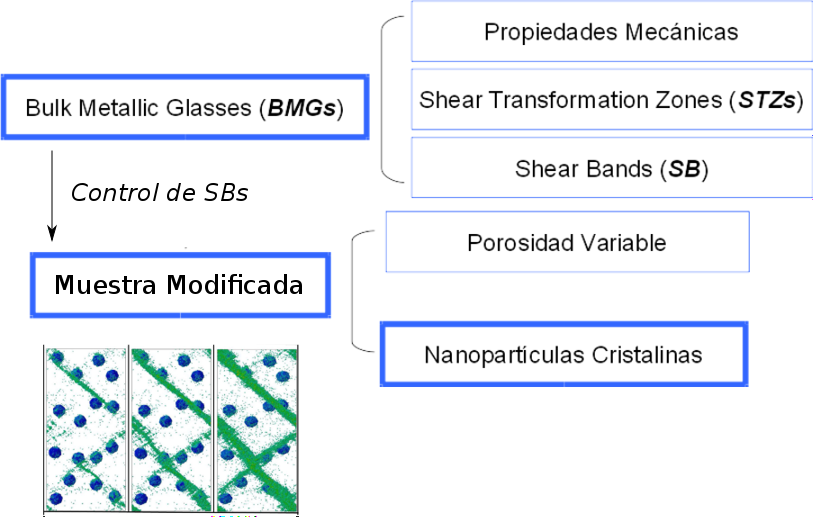
\includegraphics[width=11cm]{Presentacion/modifications_A.png}
    \end{figure}
  \end{textblock*}

%   \begin{itemize}
%    \item Para homogeneizar el r\'egimen pl\'astico y evitar la falla fr\'agil del material, la composici\'on se modifica de diferentes maneras
%   \end{itemize}
%   \begin{textblock*}{12.6cm}(-0.1cm, 3cm)  
%     \begin{figure}[htp]
%       \centering
%       \begin{tabular}{c}
% 	\subfloat[Nanopart\'iculas (Albe et al, 2013)]{
% 		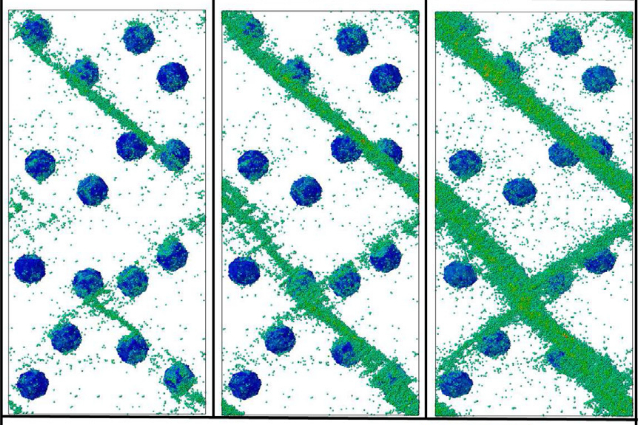
\includegraphics[width=5.7cm]{Presentacion/nanoparticles_example.png}
% 		\label{P:fg:B2Crystal}}
% 	\hspace{0.5cm}
% 	\subfloat[Nanovidrios (Adibi et al, 2013)]{
% 		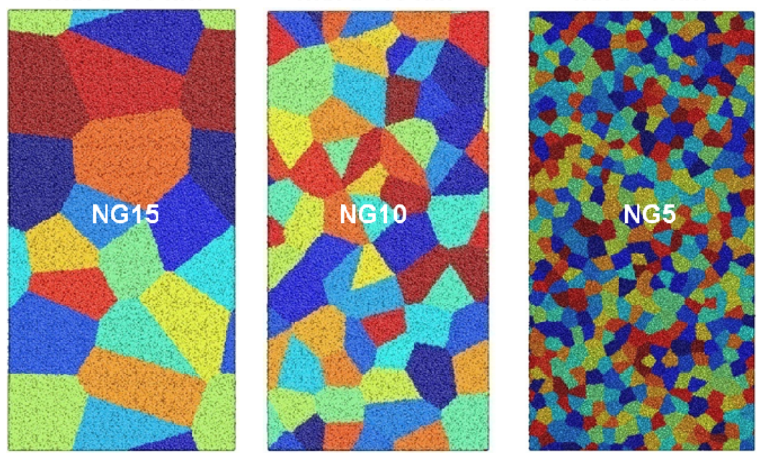
\includegraphics[width=6cm]{Presentacion/nanoglass_example.png}
% 		\label{P:fg:B2CrystalTest}}
%       \end{tabular}
%     \end{figure}
%   \end{textblock*}
  \begin{textblock*}{4.5cm}(5.5cm,8.3cm)
  \scriptsize{Albe, K., Ritter, Y., and Şopu, D., \textit{Mech. Mater.}, \textbf{67}, 94–103 (2013)}
%   Adibi, S., Sha, Z., Branicio, P., Joshi, S., Liu, Z., and Zhang, Y., \textit{Appl. Phys. Lett.}, \textbf{103}, 211905 (2013).\\
  \end{textblock*}
\end{frame}

\begin{frame}
\frametitle{Objetivos del estudio}
\vspace{0.5cm}
 \vspace{0.5cm}
 \begin{itemize}
  \item Estabilidad t\'ermica de las nanopart\'iculas (difusi\'on del material cristalino en la matriz amorfa).
  \vspace{0.5cm}
  \item Impacto en el comportamiento mec\'anico de la muestra (cambios en curvas tensi\'on-deformaci\'on)
  \vspace{0.5cm}
  \item Distribuci\'on de la deformaci\'on at\'omica de la muestra.
 \end{itemize}
\end{frame}

\begin{frame}
 \frametitle{Detalles de la simulaci\'on}
 \vspace{0.3cm}
 \begin{itemize}
  \item Muestra original ya caracterizada: Cu$_{46}$Zr$_{54}$ - 160k \'atomos
  \item Condiciones de bordes peri\'odicas en las tres dimensiones
  \item Nanopart\'iculas: Esferas de 2 nm de radio de composici\'on (a) Cu-FCC y (b) CuZr-B2
  \item La constante de red del cobre se establece en 0.3615 nm
  \item La estructura CuZr-B2 se genera ad-hoc para la simulaci\'on y da como resultado una constante de 0.3283 nm
  \item Velocidad de deformaci\'on de 10$^{9}$/s
 \end{itemize}
\end{frame}

% \begin{frame}
%  \frametitle{Preparaci\'on de cristal CuZr-B2}
%   \begin{itemize}
%     \item Cubo cristalino aislado de 15 celdas unitarias de ancho
%     \item Constante de celda de 3.50 \AA{} \cite{inoue04}
%     \item PBC en las tres dimensiones
%     \item Minimizado de energ\'ia y relajaci\'on a presi\'on cero.
%     \item T$_{i}$ = 1100 K \cite{pauly10} (988 K $\leq$ T$_{B2}$ $\leq$ 1200 K)
%     \item Se equilibra a P = 0 y T = T$_{B2}$ en 100 ps
%     \item Recocido a T = T$_{B2}$ por 150 ps
%     \item Enfriado r\'apido a 10$^{12}$ K/s hasta 300 K
%   \end{itemize}
% \end{frame}
% \begin{frame}
%   \frametitle{Preparaci\'on de cristal CuZr-B2}
%   \begin{textblock*}{12cm}(0cm,3cm)
%     \begin{table}[htp]
%     \begin{center}
%     \begin{tabular}{*{2}{c}}
%     \hline
%     Velocidad de enfriamiento [K/s] & 10$^{12}$ \\
%     \hline
%     N\'umero de \'atomos & 6750 \\
%     \hline
%     Constante de celda [\AA] & 3.283 \\
%     \hline
%     Energ\'ia total (eV) & -34012.8 \\
%     \hline
%     Energ\'ia de cohesi\'on (eV) & -5.04 \\
%     \hline
%     \end{tabular}
%     \end{center}
%     \end{table}
%   \end{textblock*}
%   
%   \begin{textblock*}{12cm}(0cm,7cm) 
%     \centering
%       Par\'ametros obtenidos para el cristal CuZr (B2)
%   \end{textblock*}
% \end{frame}
\begin{frame}
  \frametitle{Preparaci\'on de cristal CuZr-B2}
    \begin{textblock*}{12.6cm}(-0.08cm,1.5cm) 
      \begin{figure}[htp]
	\centering
	\subfloat[Cristal]{
	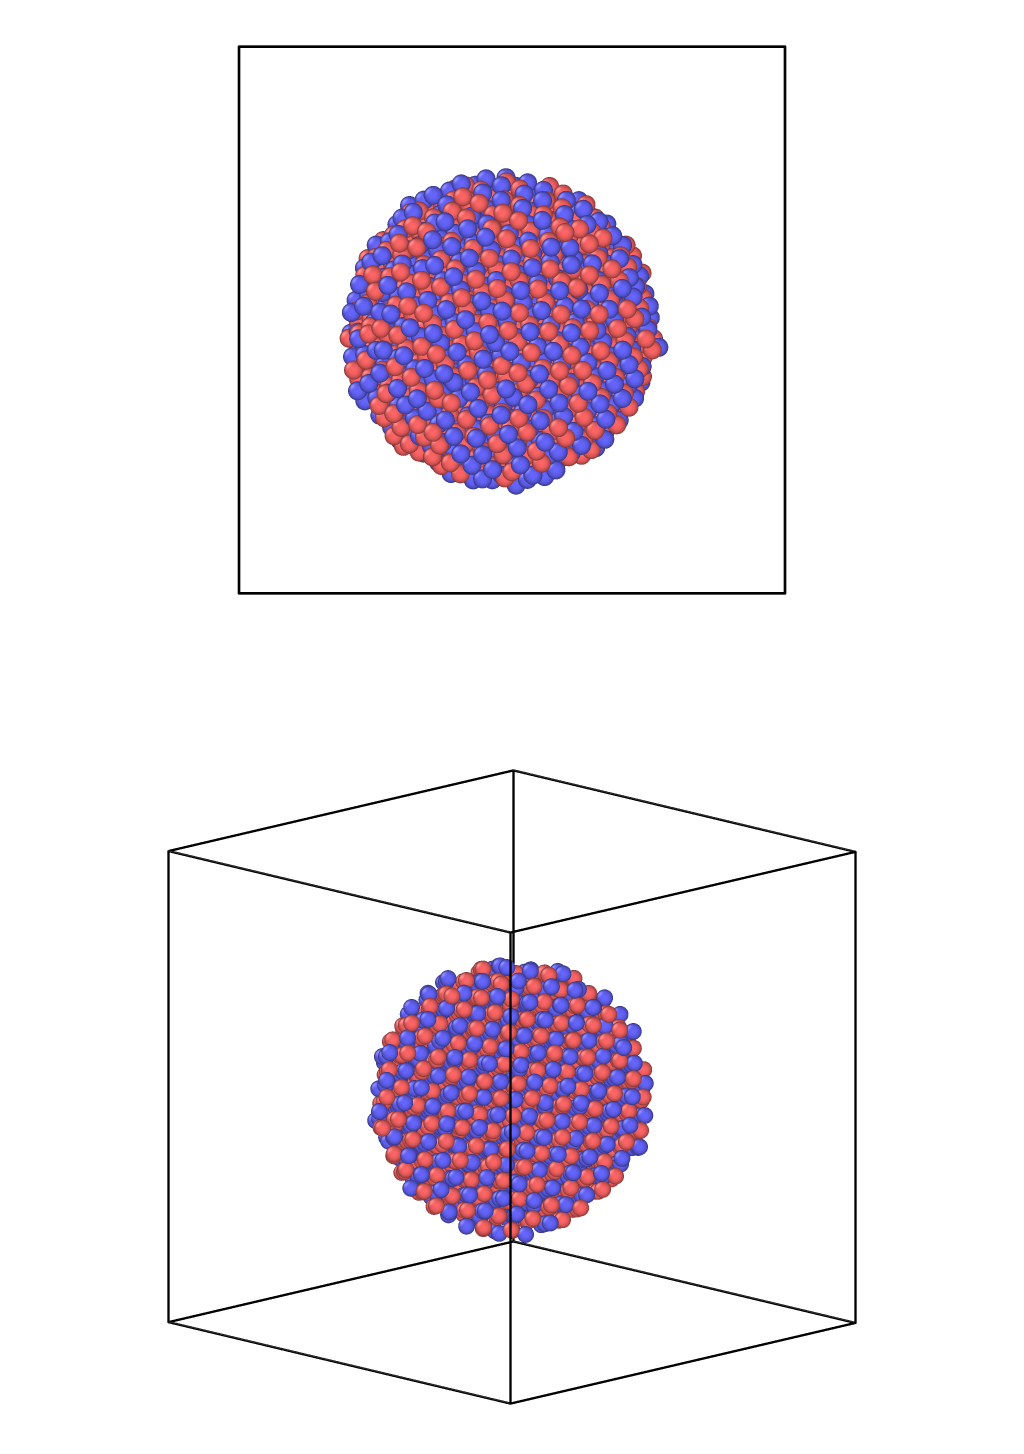
\includegraphics[height=5cm]{Cap_4/B2_FreeBoundaries.png}}
	\subfloat[Energ\'ia de cohesi\'on vs tiempo]{
	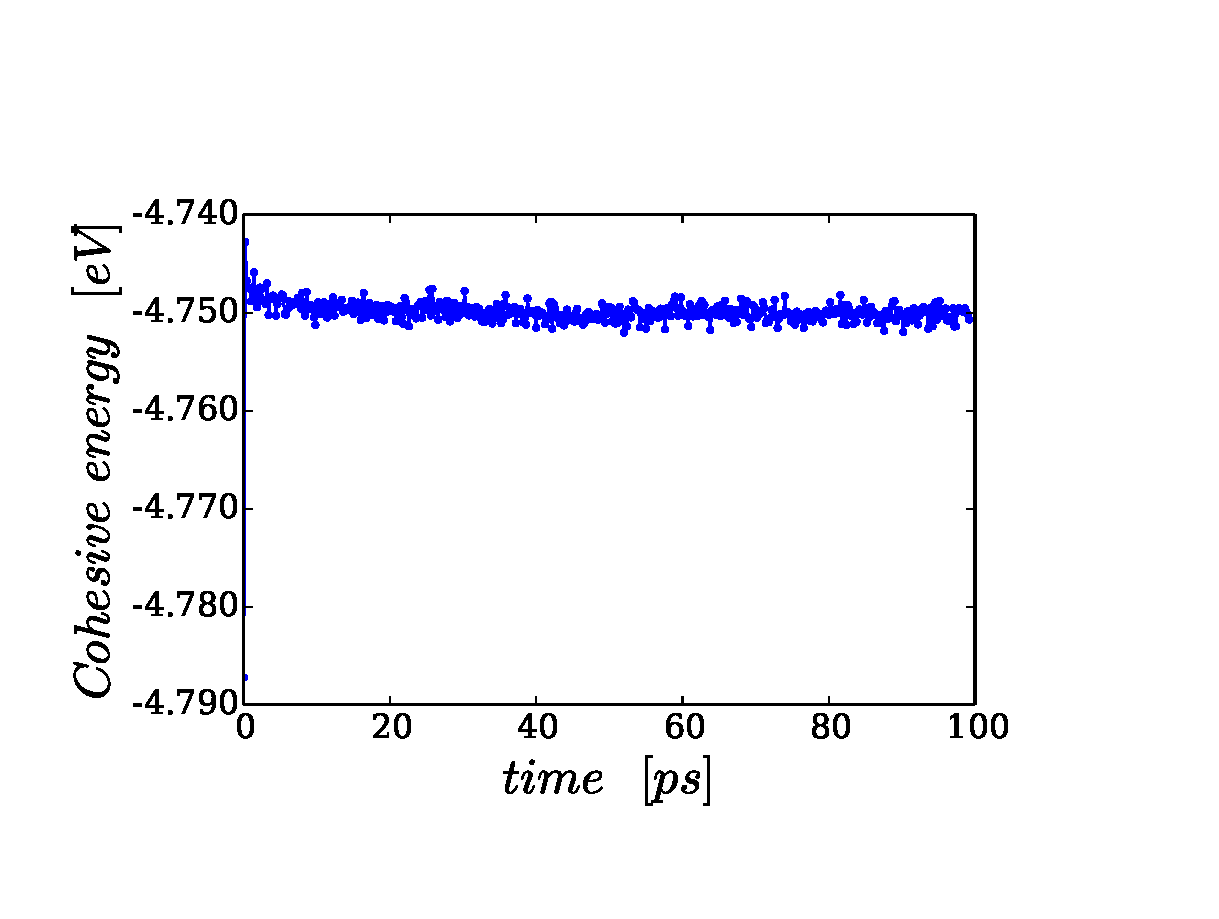
\includegraphics[width=6.3cm]{Cap_4/B2CrystalTest_FreeBoundariesSphere.pdf}}
      \end{figure}
    \end{textblock*}
    \begin{textblock*}{10cm}(1.5cm,8.5cm) 
    \centering
      Verificaci\'on del cristal CuZr-B2
  \end{textblock*}
\end{frame}

% \begin{frame}
%  \frametitle{Vista de la muestra preparada}
%  
%  \begin{textblock*}{12.6cm}(-0.08cm,1.5cm) 
%      \begin{figure}[htp]
% 	\centering
% 	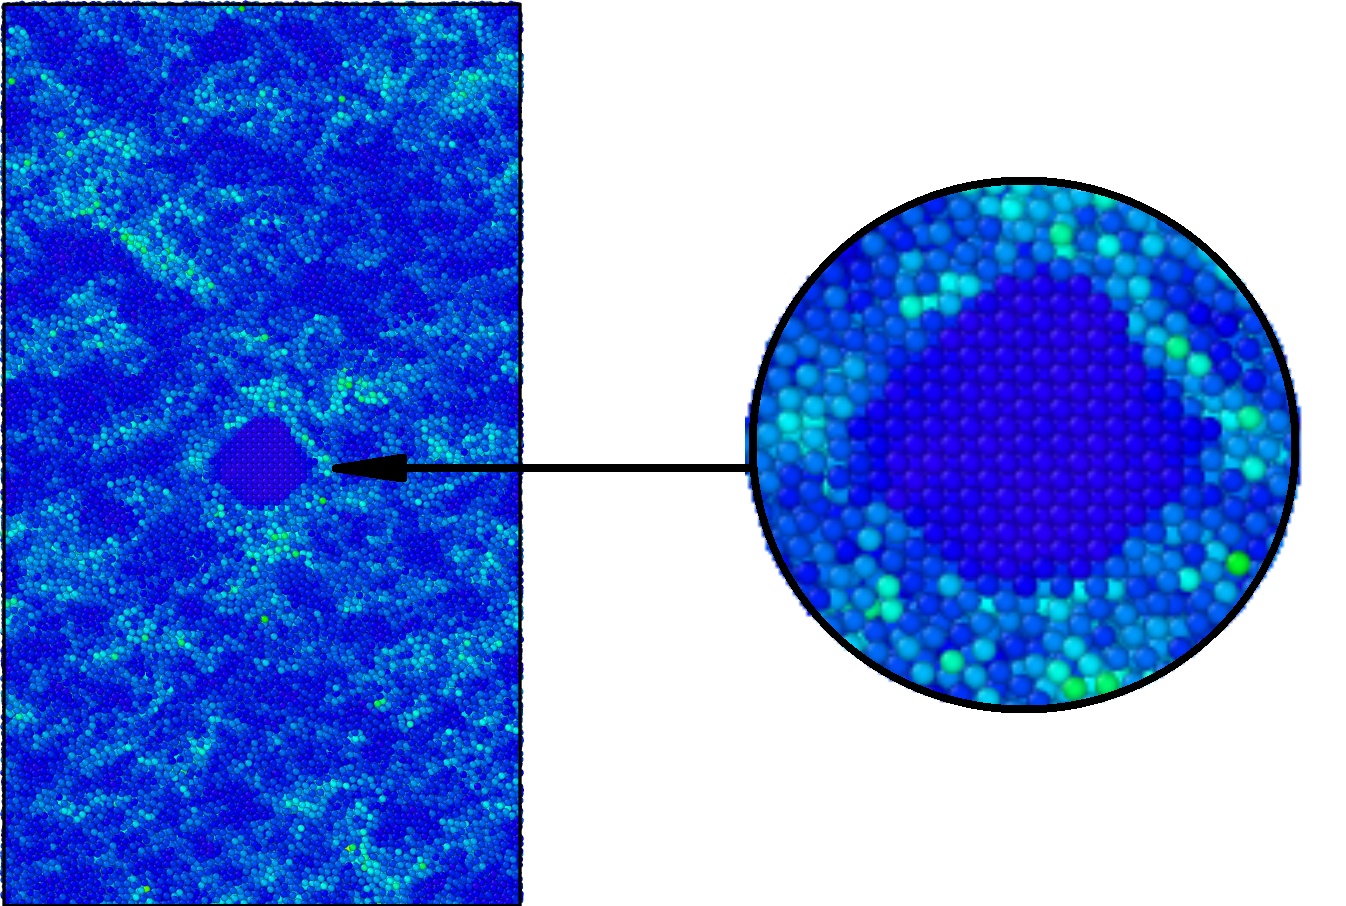
\includegraphics[height=6cm]{Cap_4/NP_CloseUp_FCC.png}
%       \end{figure}
%   \end{textblock*}
%  
% \end{frame}

\begin{frame}
 \frametitle{Resultados}
 
 \begin{textblock*}{12.6cm}(-0.08cm,1.5cm) 
      \begin{figure}[htp]
	\centering
	\subfloat[Bajas Temperaturas]{
	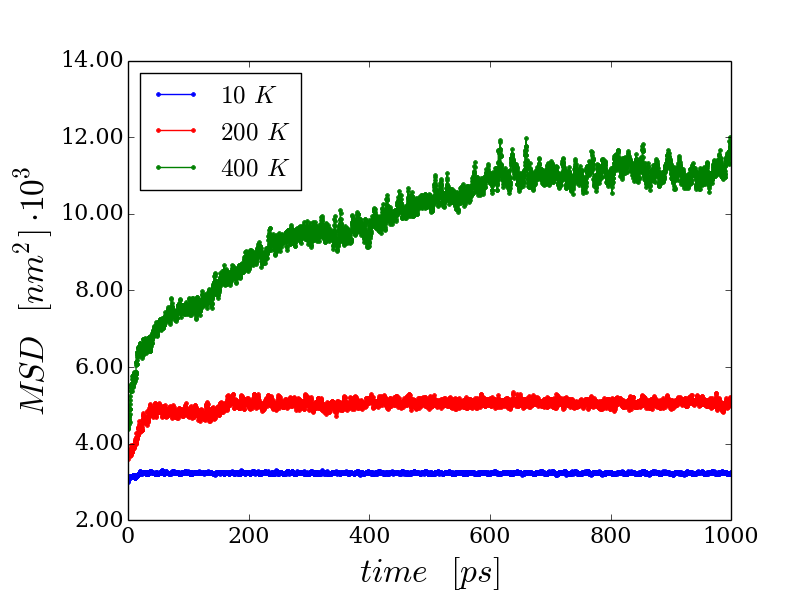
\includegraphics[width=6.3cm]{Cap_4/msd10_400_FCC.png}}
	\subfloat[Altas Temperaturas]{
	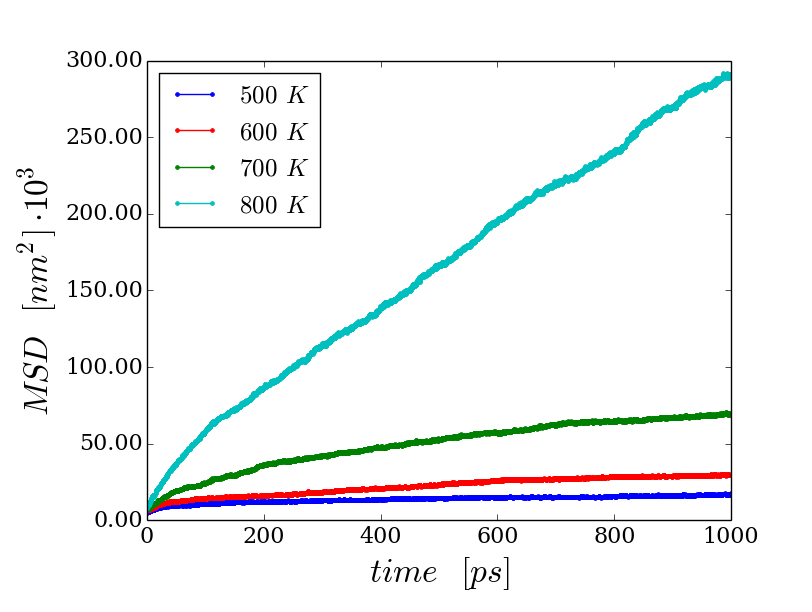
\includegraphics[width=6.3cm]{Cap_4/msd500_800_FCC.png}}
      \end{figure}
    \end{textblock*}
    \begin{textblock*}{10cm}(1.5cm,8cm) 
    \centering
      Desplazamientos cuadr\'aticos medios para la nanopart\'icula Cu-FCC
 \end{textblock*}
\end{frame}

\begin{frame}
 \frametitle{Resultados}
 
 \begin{textblock*}{12.6cm}(-0.08cm,1.5cm) 
      \begin{figure}[htp]
	\centering
	\subfloat[Bajas Temperaturas]{
	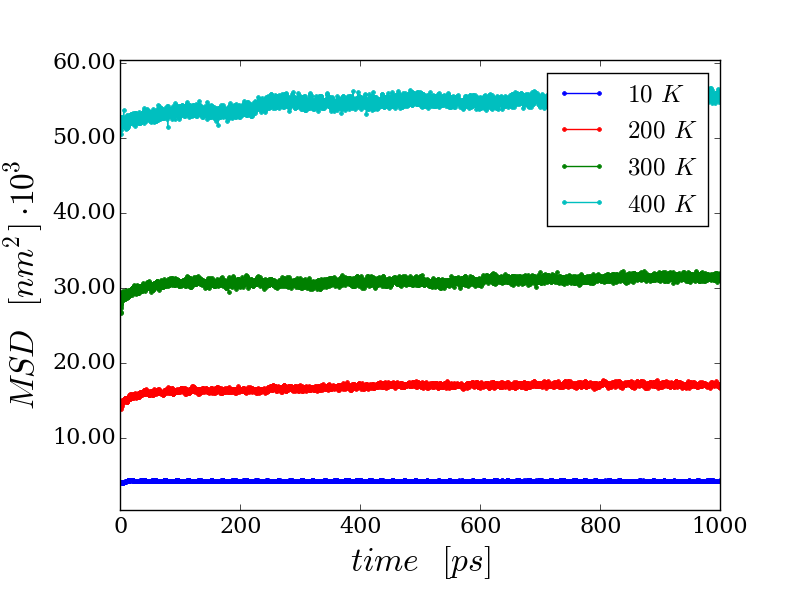
\includegraphics[width=6.3cm]{Cap_4/msd10_400_B2.png}}
	\subfloat[Altas Temperaturas]{
	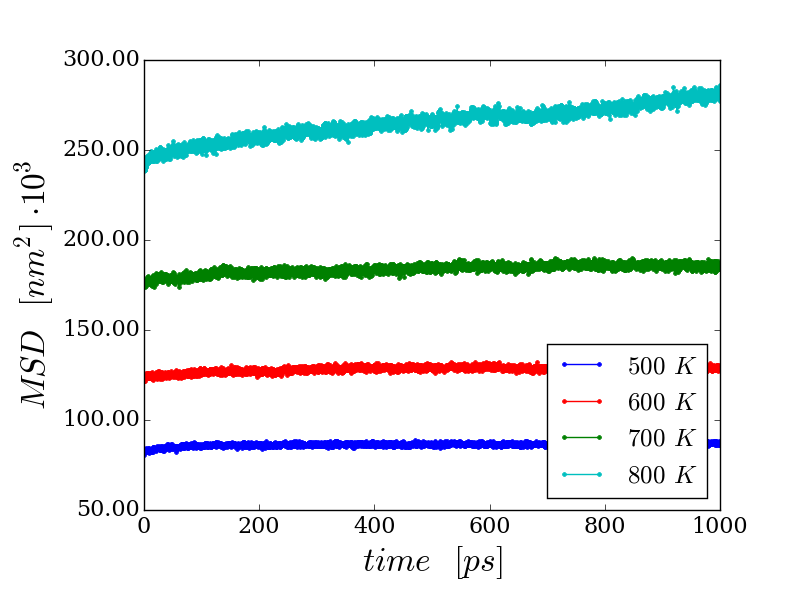
\includegraphics[width=6.3cm]{Cap_4/msd500_800_B2.png}}
      \end{figure}
    \end{textblock*}
    \begin{textblock*}{10cm}(1.5cm,8cm) 
    \centering
      Desplazamientos cuadr\'aticos medios para la nanopart\'icula CuZr-B2
 \end{textblock*}
\end{frame}

\begin{frame}
 \frametitle{Resultados}
 
  \begin{textblock*}{6.5cm}(-0.08cm,2cm) 
   \begin{figure}[htp]
    \centering
    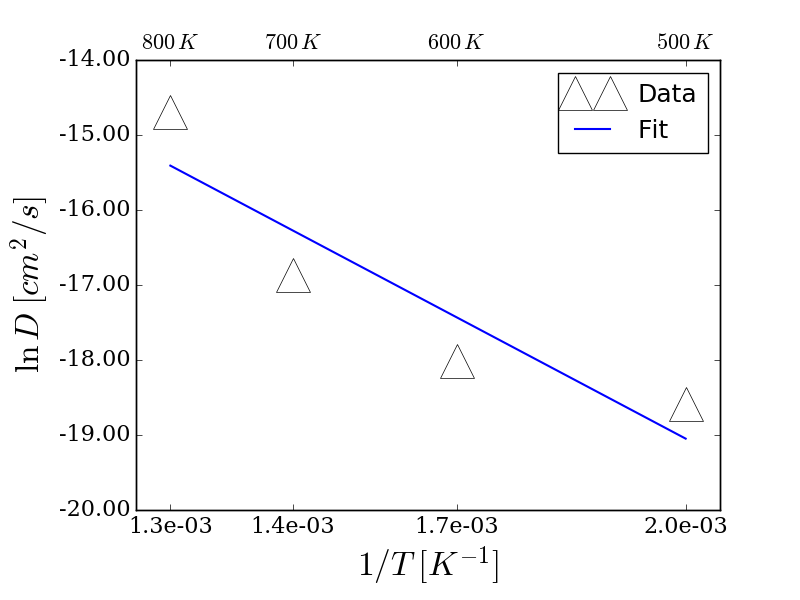
\includegraphics[width=6.3cm]{Cap_4/FCCDiff_vs_temp_fit.png}
   \end{figure}
  \end{textblock*}
  \begin{textblock*}{12cm}(0.2cm,8.5cm) 
    \centering
    Difusividad en funci\'on de la temperatura para el caso Cu-FCC
  \end{textblock*}
  
  \begin{textblock*}{6cm}(6.5cm,3cm)
    Modelo usado: \\
    \vspace{0.5cm}
    $D = D_{0}\cdot \mathrm{e}^{\frac{-\Delta E}{k_{B} T}}$\\
    \vspace{0.5cm}
    Resultados de la regresi\'on:
    \begin{table}[htp]
      \begin{center}
      \begin{tabular}{*{2}{c}}
      \hline
      $\Delta E$ [$eV$]& $-0,4182$ \\
      \hline
      D$_{0}$ [$\frac{nm^{2}}{ps}$] & $8,771\times 10^{-3}$\\
      \hline
      R$^{2}$ & 0.8399 \\
      \hline
      \end{tabular}
      \end{center}
      \end{table}    
  \end{textblock*} 
\end{frame}

\begin{frame}
 \frametitle{Carga uniaxial del BMG}
  \begin{textblock*}{12.6cm}(-0.08cm,1.5cm) 
      \begin{figure}[htp]
	\centering
	\subfloat[Tracci\'on]{
	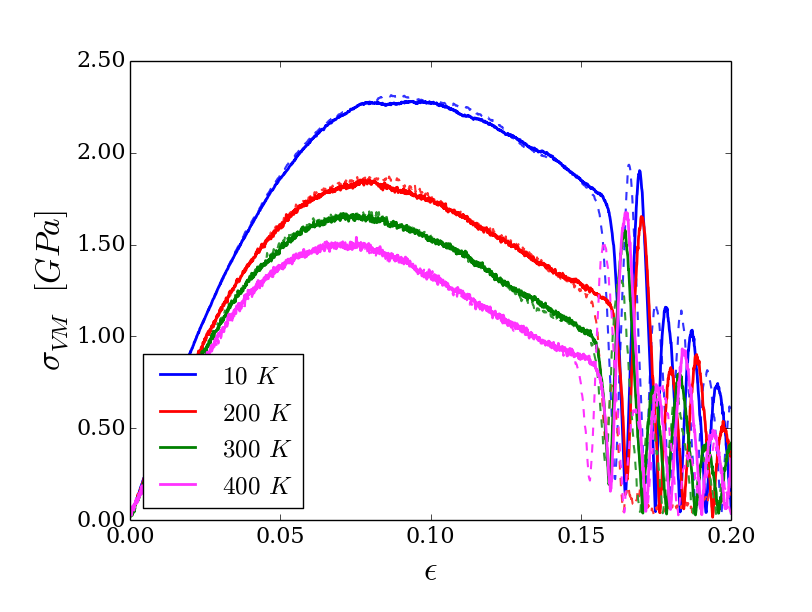
\includegraphics[width=6.3cm]{Cap_4/stress_strain_tension_FCC_NoInc.png}}
	\subfloat[Compresi\'on]{
	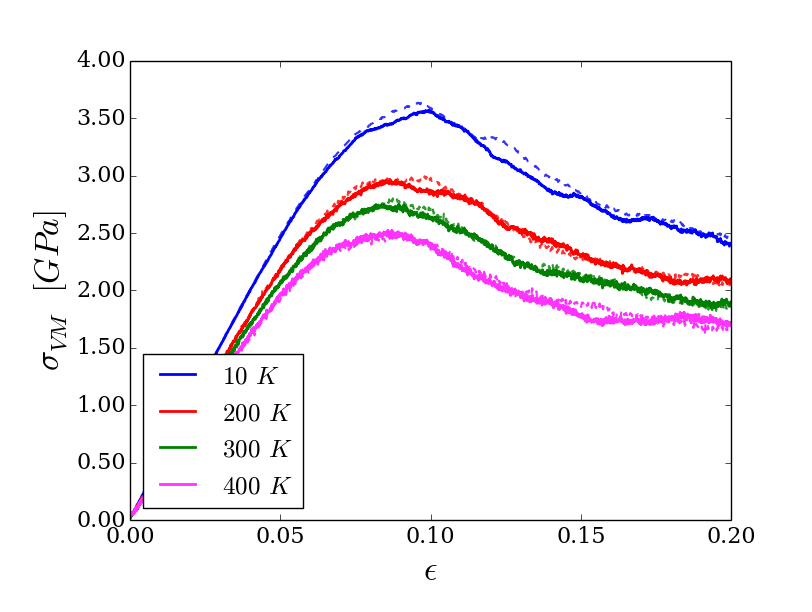
\includegraphics[width=6.3cm]{Cap_4/stress_strain_compression_FCC_NoInc.png}}
      \end{figure}
    \end{textblock*}
    \begin{textblock*}{12cm}(0.5cm,8.2cm) 
    \centering
      Tensi\'on de Von Mises vs deformaci\'on para el BMG sin inclusi\'on (l\'inea punteada) y una inclusi\'on de Cu-FCC (l\'inea s\'olida)
    \end{textblock*}
\end{frame}
\begin{frame}
  \frametitle{Carga uniaxial del BMG}
    \begin{textblock*}{12.6cm}(-0.08cm,1.5cm) 
      \begin{figure}[htp]
	\centering
	\subfloat[Tracci\'on]{
	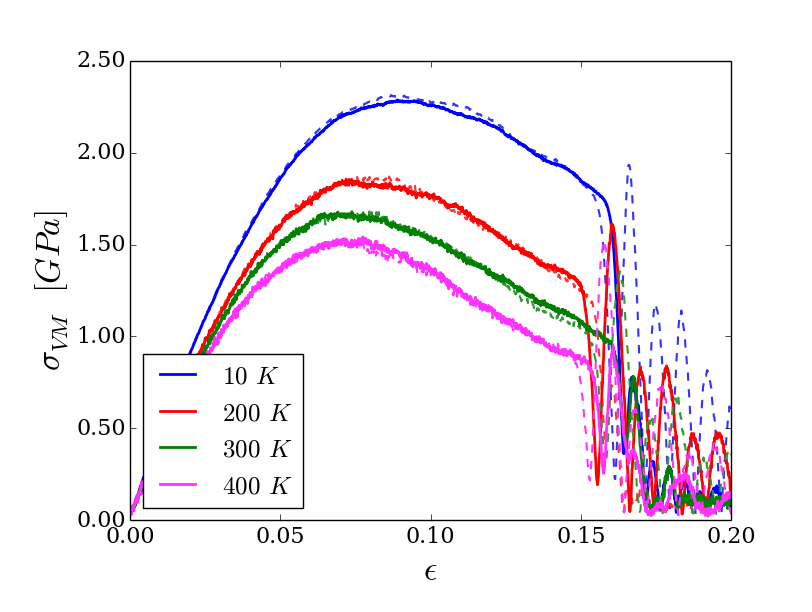
\includegraphics[width=6.3cm]{Cap_4/stress_strain_tension_B2_NoInc.png}}
	\subfloat[Compresi\'on]{
	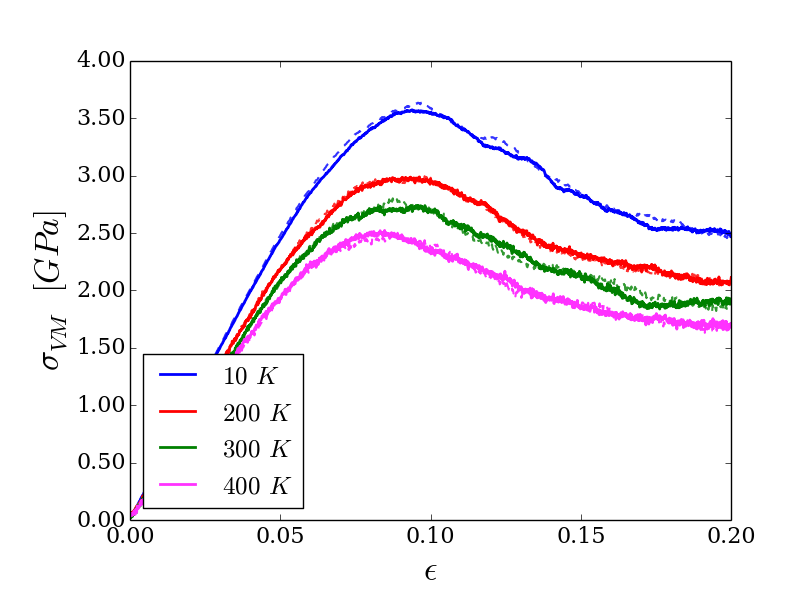
\includegraphics[width=6.3cm]{Cap_4/stress_strain_compression_B2_NoInc.png}}
      \end{figure}
    \end{textblock*}
    \begin{textblock*}{12cm}(0.5cm,8.2cm) 
    \centering
      Tensi\'on de Von Mises vs deformaci\'on para el BMG sin inclusi\'on (l\'inea punteada) y una inclusi\'on de CuZr-B2 (l\'inea s\'olida)
    \end{textblock*}
\end{frame}

\begin{frame}
  \frametitle{Cortes de la muestra}
  \begin{textblock*}{12.6cm}(-0.08cm,1.5cm) 
    \begin{figure}[htp]
     \centering
     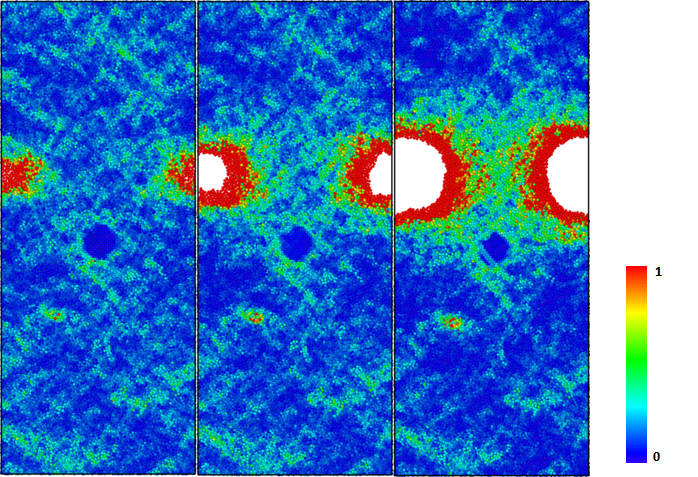
\includegraphics[height=6cm]{cuSphereTension_10K_Snapshots.png}
    \end{figure}
  \end{textblock*}
  \begin{textblock*}{12cm}(0.5cm,8.5cm) 
    \centering
      \small{Inclusi\'on de Cu-FCC bajo tracci\'on a 10K según deformaci\'on atómica. De izquierda a derecha: $\epsilon$ = 16.66 \%, 16.68 \% y 16.70 \%.}
    \end{textblock*}
    
   \only<2>{
    \begin{textblock*}{10cm}(6cm,2cm)
      \begin{figure}[htp]
	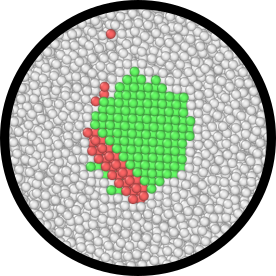
\includegraphics[width=3cm]{Presentacion/nanoparticles_macla.png}
    \end{figure}
    \end{textblock*}
   }
\end{frame}

\begin{frame}
  \frametitle{Cortes de la muestra}
  \begin{textblock*}{12.6cm}(-0.08cm,1.5cm) 
    \begin{figure}[htp]
     \centering
     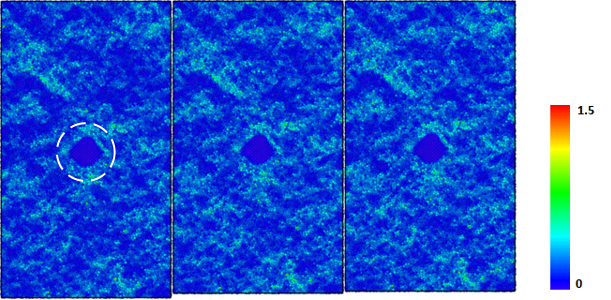
\includegraphics[height=6cm]{cuSphereCompression_10K_Snapshots.png}
    \end{figure}
  \end{textblock*}
  \begin{textblock*}{12cm}(0.5cm,8.5cm) 
    \centering
      \small{Inclusi\'on de Cu-FCC bajo compresi\'on a 10K según deformaci\'on atómica. De izquierda a derecha: $\epsilon$ = 16.74 \%, 16.86 \% y 16.92 \%.}
    \end{textblock*}
\end{frame}

\begin{frame}
  \frametitle{Cortes de la muestra}
  \begin{textblock*}{12.6cm}(-0.08cm,1.5cm) 
    \begin{figure}[htp]
     \centering
     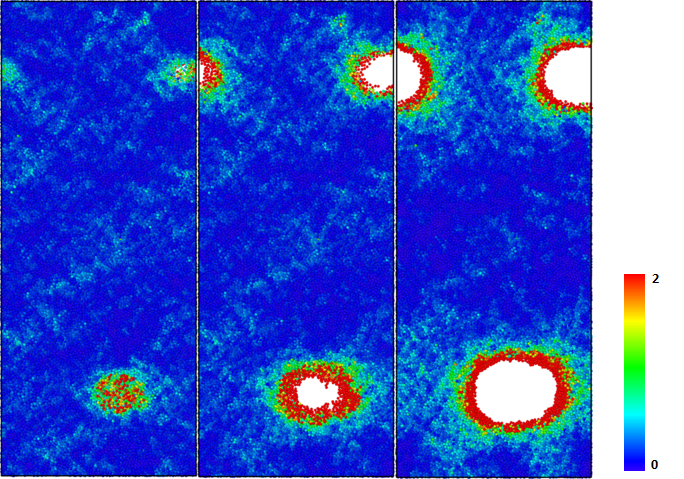
\includegraphics[height=6cm]{B2SphereTension_10K_Snapshots.png}
    \end{figure}
  \end{textblock*}
  \begin{textblock*}{12cm}(0.5cm,8.5cm) 
    \centering
      \small{Inclusión de CuZr-B2 bajo tracción a 10K según deformación atómica. De izquierda a derecha: $\epsilon$ = 16.66 \%, 16.68 \% y 16.70 \%.}
    \end{textblock*}
\end{frame}

\begin{frame}
  \frametitle{Cortes de la muestra}
  \begin{textblock*}{12.6cm}(-0.08cm,1.5cm) 
    \begin{figure}[htp]
     \centering
     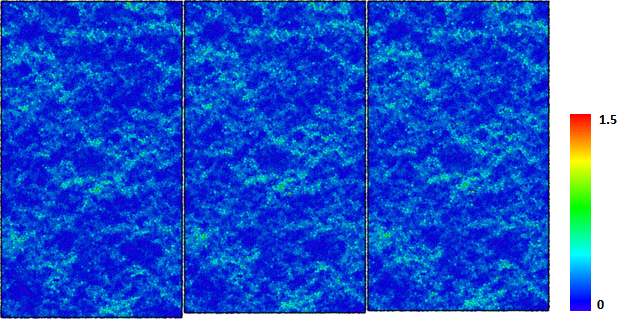
\includegraphics[height=6cm]{B2SphereCompression_10K_Snapshots.png}
    \end{figure}
  \end{textblock*}
  \begin{textblock*}{12cm}(0.5cm,8.5cm) 
    \centering
      \small{Inclusión de CuZr-B2 bajo compresión a 10K según deformación atómica. De izquierda a derecha: $\epsilon$ = 16.74 \%, 16.86 \% y 16.92 \%.}
    \end{textblock*}
\end{frame}

